\documentclass[a4paper,12pt,bibliography=totoc,index=totoc,twoside,francais]{scrbook}
%\documentclass[a4paper,12pt,DIVcalc,bibliography=totoc,index=totoc,twoside,francais]{scrbook}
\KOMAoptions{titlepage,chapterprefix,open=right}
%\KOMAoptions{bibliography=totoc,index=totoc}
%\addtokomafont{chapter}{\rmfamily}
%\addtokomafont{section}{\rmfamily}

\usepackage[utf8]{inputenc}
\usepackage[T1]{fontenc}
\usepackage{lmodern}
\usepackage{graphicx}
\usepackage[automark,headsepline]{scrpage2}
\usepackage[style=numeric,sorting=none,backend=biber]{biblatex}
\usepackage{csquotes}
\usepackage{xspace}
\usepackage[autolanguage]{numprint}
\usepackage{array}
\usepackage{booktabs}
\usepackage[table,svgnames,dvipsnames]{xcolor}
\usepackage[final]{pdfpages} 
\clubpenalty=5000
\widowpenalty=5000

%\usepackage{lipsum}
%\bibliography{biblio}

\usepackage[backend=biber]{biblatex}
\addbibresource{biblio.bib}

%\usepackage{hyperref} 
\usepackage[pdfauthor={Cynthia Lopes do Sacramento}, pdftitle={SDN : Software-Defined Networking}]{hyperref}

\usepackage{makeidx}
\makeindex


%\usepackage[xindy={language=french,codepage=utf8},acronym,toc=true,nonumberlist]{glossaries}
%\usepackage[acronym,toc=true,nonumberlist]{glossaries}
\usepackage[toc=true,acronym,nopostdot,nonumberlist]{glossaries}
%\usepackage[toc=true,acronym]{glossaries}

\makeglossaries


\let\Oldgls\gls%Transformation de la commande \gls en \Oldgls
\let\Oldglslink\glslink%Transformation de la commande \gls en \Oldgls
\let\Oldglspl\glspl%Transformation de la commande \gls en \Oldgls

% Création de la nouvelle commande \gls
\renewcommand{\gls}[1]{%
\textbf{ \Oldgls{#1}} 
}
% Création de la nouvelle commande \gls
\renewcommand{\glslink}[2]{%
\textbf{ \Oldglslink{#1}{#2}} 
}
% Création de la nouvelle commande \gls
\renewcommand{\glspl}[1]{%
\textbf{ \Oldglspl{#1}} 
}

\newacronym{rtfm}{RTFM}{Read the f\dots manual}

\newacronym{sdn}{SDN}{Software-Defined Networking, Réseau Informatique Défini par Logiciel}

\newacronym{ti}{TI}{Technologie de l'Information}

\newacronym{si}{SI}{Système d'Information}

\newacronym{nfv}{NFV}{Network Functions Virtualization, Virtualisations des fonctions réseau}



\newglossaryentry{paradigme}
{
  name=Paradigme,
  description={Un paradigme dénote une collection de règles, standards et exemples de pratiques scientifiques, partagés par un groupe de scientifiques. 
  Sa genèse et continuation de la tradition de recherche sont conditionnées à l'engagement et au consensus qui en découle. \cite{paradigmdef}
  D'après Dosi \cite{newparadigm}, quand un nouveau paradigme technologique apparaît, il représente une discontinuité ou un changement de la manière de penser. Ce changement apporté par le paradigme est souvent lié à une sorte d'innovation radicale qui applique une nouvelle technologie. Dans ce document, le terme paradigme sera employé dans ce sens d'innovation et application de nouvelle technologie    }
}


\newglossaryentry{bigdata}
{
  name=Big Data,
  description={Big Data est un terme appliqué aux ensemble de données dont la taille est au-delà de la capacités des outils logiciels communs de les capturer, gérer et traiter. Une nouvelle classe de technologies et outils ont été développés pour surmonter le challenge de créer valeur commercial à partir la complexe analyse de ces donnés. Le terme est employé pour référer ce type de données ainsi que les technologies utilisées pour les stocker et traiter
  \cite{IMBigData}    }
}


\newglossaryentry{cloudcomputing}
{
  name=Cloud Computing,
  description={  Le  Cloud Computing est x }
}
\newglossaryentry{virtualisation}
{
  name=Virtualisation,
  description={  La Virtualisation  est y  }
}
\newglossaryentry{datacenter}
{
  name=Data  Center,
  description={  Centre de données.  }
}
\newglossaryentry{middlebox}
{
  name=Middlebox,
  description={  Boîtier intermédiaire. Un middlebox est un serveur gardant des états au milieu de la communication entre deux hôtes. Ils se différencient des hôtes qui représentent les 'endpoints' de la communication. Ils sont encore différents des routeurs qui ne gardent pas d'états concernant les instances de communications.   },
  plural=Middleboxes
}


\usepackage[english,francais]{babel}
\frenchbsetup{og=«, fg=»}



\pagestyle{scrheadings}

\begin{document}
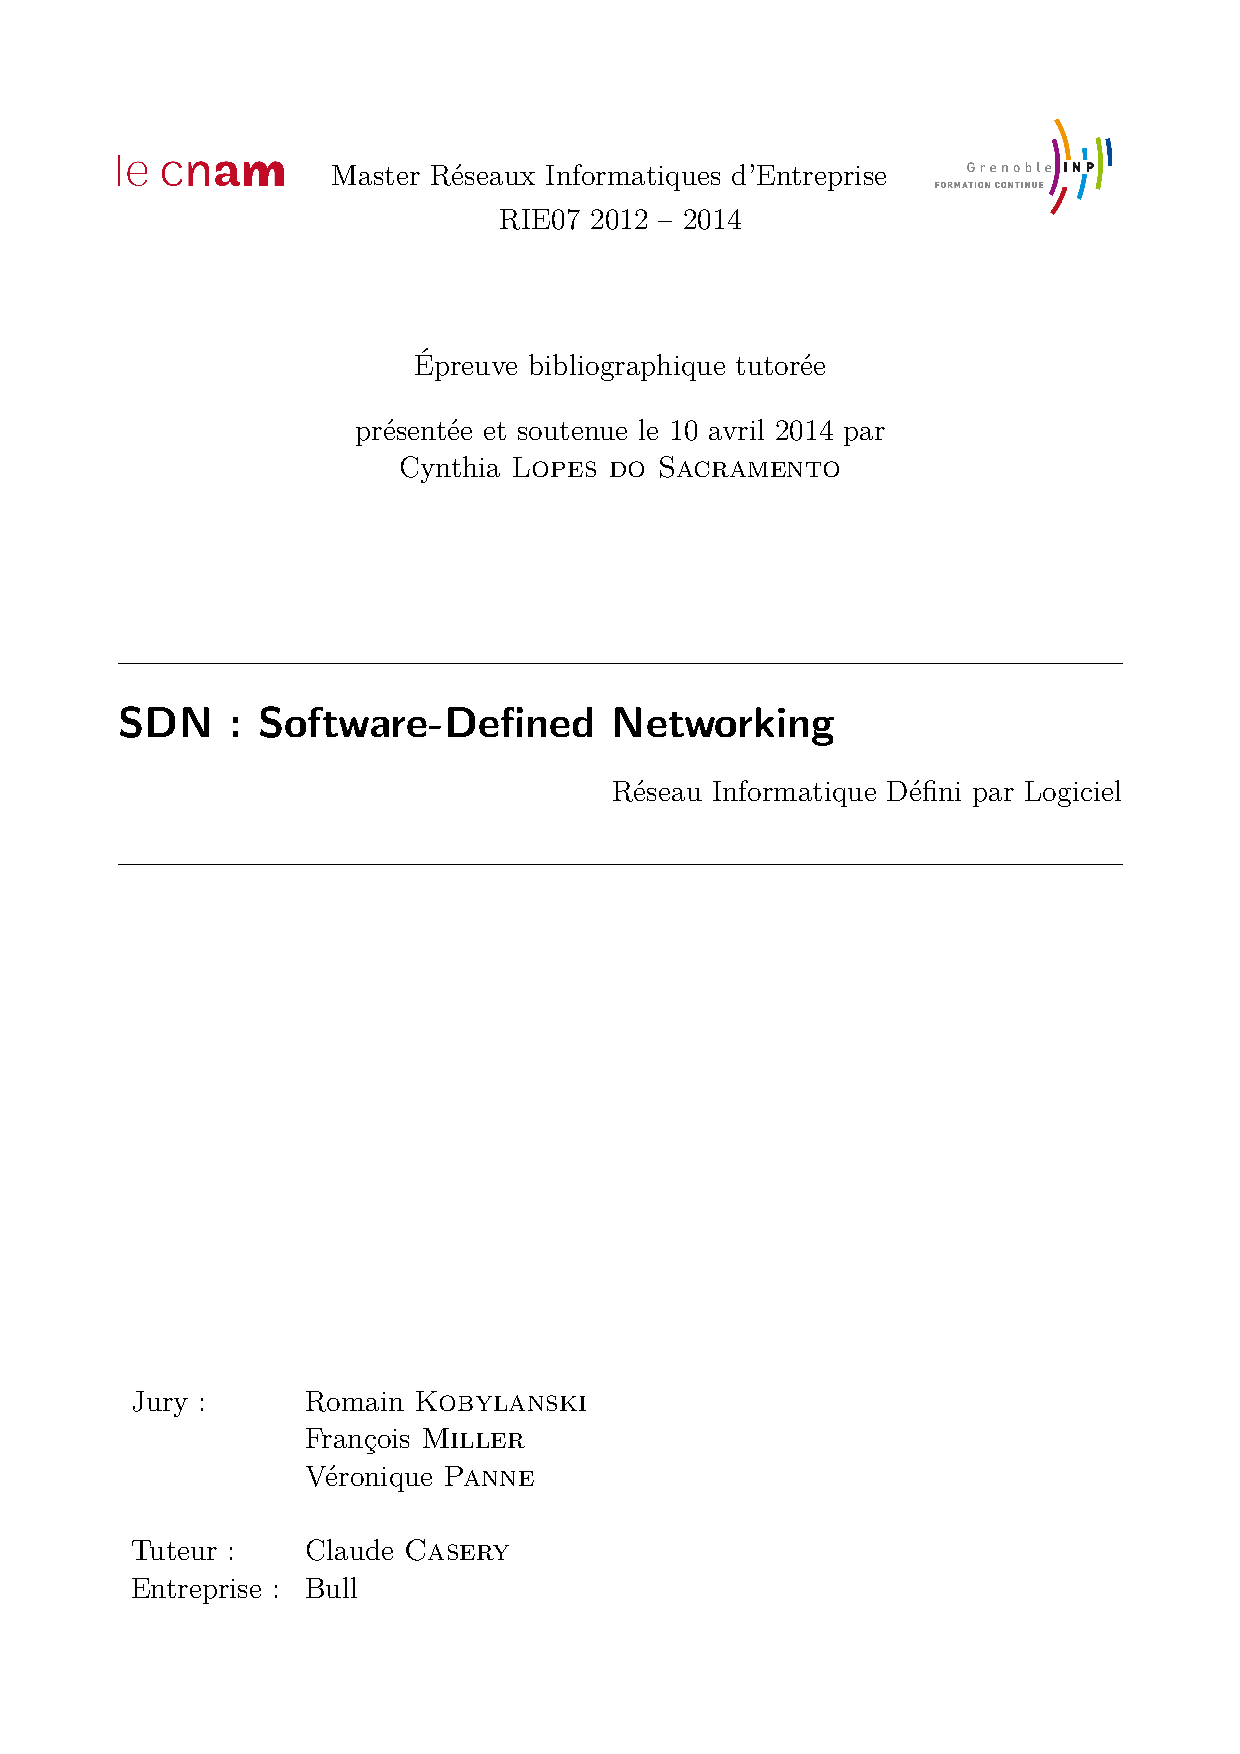
\includepdf[pages={1-2}]{couverture-ebt.pdf}

\frontmatter
\begin{flushright}
It is harder to crack a prejudice than an atom.\\
Albert \bsc{Einstein}\\
\end{flushright}

\tableofcontents
\listoftables
\listoffigures

\mainmatter
%\addchap{Introduction}
\addchap{Introduction}

%\section{To Do}
%Parler de la croissance (de l'explosion même) de l'utilisation de l'internet. Du hypertexte aux applications dynamiques. Puis la virtualisation et le cloud computing. Ensuite le big data. Montrer que ça évolue en grande vitesse.
%\par Expliquer que l'architecture et l'infrastructure réseau n'avaient pas été conçues pour ce scénario. Donc ça commence à se saturer ne correspondant plus aux besoins actuels. Les choses sont plus éphémères, il y a besoin de quelque chose plus flexible, adaptable. Et l'architecture actuelle pose des difficultés pour l'expérimentation des nouveaux protocoles, services, applications etc. 
%\par Introduire SDN comme une réponse à cette problématique. Expliquer brièvement ce que c'est et pour quoi cela apporte une évolution. Montrer comment ça pourrait être utilisé pour répondre aux besoins actuels.
%\par Expliquer les objectifs du texte : ré-définir SDN, présenter les enjeux et les cas d'utilisation et un état de l'art des technologies qui sont sorties.
%\par Présenter la méthodologie, le développement du texte et de quoi va parler chaque section. 
 

%\section{Évolution de l'utilisation Internet pendant une décade}

[3 lignes qui parlent de SDN et utilisent les mots clefs du sujet.]

L'internet a évolué de trois manières importantes dans les dix dernières années. 
\begin{itemize}
\item Le contenu a évolué de texte et pages web relativement statiques, il a progressé vers un contenu multimédia haut-débit exigeant une latence réduite. 
\item L'utilisation s'est rapidement mondialisée; par exemple le débit international servant l'Afrique a augmenté de 1.21Gbit/s en 2001 à 570.92Gbit/s en 2011 \cite{InternetGlobalGrowthImpactDevelopingCountries}.
\item  L'accès a étendu des ordinateurs de bureau à une variété de nouveaux dispositifs, comme pour les téléphones mobiles dont le trafic global des donnés a augmenté de 70\% en 2012. \cite{CiscoVNI2013}. 
\end{itemize}
Fait important: la rapidité d'une telle évolution technologique et son adoption est sans précédent dans l'histoire de l'humanité. 


\par
La capacité d'évolution pour s'adapter aux nouvelles exigences des usagers est recourrente dans l'histoire de l'Internet. 
%La croissance accélérée de l'accès de partout, notamment dans les pays en développement et la rapide augmentation de l'utilisation par les utilisateurs existants, dirigées par les contenus multimédias et application machine-à-machine sont des 
En revanche, dans le scénario actuel on voit poindre une croissance accélérée de l'accès de partout, notamment dans les pays en développement, ainsi qu'une rapide augmentation de l'utilisation par les utilisateurs existants, engendrée par les contenus multimédias et les applications machine-à-machine. Par exemple, en moins de deux ans depuis la parution d'Instagram, plus de 50 millions de personnes on partagé plus d'un milliard de photos desssus. \cite{deuxAnsInstagram}.
Dans ce contexte, on met en cause capacité de l'internet, comme il est, de continuer à fournir l'infrastructure nécessaire. \cite{InternetSustainGrowthIntro}
\par
De nouvelles technologies et concepts émergent pour répondre aux nouveaux besoins de ces utilisateurs qui exigent de plus en plus haut-débit et une latence réduite. Le \gls{bigdata} a modifié le traitement des données pour permettre les entreprises de gérer la quantité massive de données manipulées. \cite{IMBigData} Le \gls{cloudcomputing} et la \gls{virtualisation} ont apporté une nouvelle approche pour le management et l'hébergement de ressources de \gls{ti} dans le but de les rendre plus agiles, plus efficaces, plus sécurisés et plus flexibles tout en réduisant les coûts. \cite{CloudComputingIntelVision}. Pour accompagner ces évolutions, une innovation technologique dans le domaine des réseaux informatiques est requise. \cite{InternetEvolutionRoleSoftwareEngineeringConclusion}
\par
Cette problématique a amené scientifiques et tout les ingénieurs impliqués dans ce secteur à la conception de \gls{sdn}. \gls{sdn} est un nouveau \glslink{paradigme}{paradigme} réseau qui est actuellement développé en collaboration pour adapter l'infrastructure existante au nouveau scénario.\cite{OpenFlowStanford} Le présent document a donc pour but d'explorer cette solution et analyser les approches qui ont été faites dans ce domaine. Il propose un état de l'art des technologies parues pour déployer \gls{sdn} ainsi que divers cas d'utilisation dont les enjeux seront présentés.
\par
[un paragraphe pour le plan du texte (de quoi parle chaque section)]
\par
[Un paragraphe pour conclure l'intro et laisser les pistes de mon point de vue et les conclusions trouvées].




\chapter{Problématique Réseau et SDN}
\label{chap-1}

%\section{Première section}\label{sec-1-1}

%\section{Deuxième section}\label{sec-1-2}

%Ce chapitre va reprendre les problèmes réseaux rencontrés pour définir les besoins actuels dans le domaine. Une liste de requis pour une architecture réseau idéalement adapté aux applications actuelles sera proposée.
%En connaissant les problèmes de l'architecture en place, la question que se pose est : si on repartait de zéro, comment on le ferrait ?

%\section{Pression pour l'expansion de l'architecture réseau }

\section{Ossification de l'internet face au besoin d'expansion}



%"The classic Internet architecture is a victim of its own success. Having succeeded so well at empowering users and encouraging innovation, it has been made obsolete by explosive growth in users, traffic, applications, and threats." The range of problems observed today is not surprising.

%The Internet was created in simpler times, among a small club of cooperating stakeholders. As the Internet becomes part of more and more aspects of society, it will inevitably be subject to more demands from more stakeholders, and be found deficient in more ways

%In the first half of the 2000s, the research climate was dominated by the belief that research is pointless unless its results can be adopted easily within the existing Internet. Attempting to work within this constraint, people realized that the current architecture makes solving some problems impossible.


À vouloir autoriser et même encourager les utilisateurs à innover sur son architecture, l'internet s'est fait dépasser par son propre succès. La croissance explosive des utilisateurs, du trafic et des applications a apporté toute une série de problèmes, 
%L'internet a été créé à une époque où les choses étaient plus simples, avec peu d'intervenants en coopération. Dès qu'il est devenu partie intégrante en plusieurs aspects de la société, diverses réclamations et défaillances sont apparues, 
tant que l'exhaustion des adresses IPv4 disponibles et les menaces aux réseaux locaux privés. 

%One of the main reasons for these security vulnerabilities is that the Internet architecture and its supporting protocols were primarily designed for a benign and trustworthy environment, with little or no consideration for security issues. This assumption is clearly no longer valid for today’s Internet, which connects millions of people, computers, and corporations in a complex web that spans the entire globe.
\par
En réponse à ces questions, on a introduit dans l'architecture des \glspl{middlebox}, par exemple les NATs et les Firewalls, à un prix : la complexité. Le logiciel dans ces systèmes est capable d'atteindre n'importe quel objectif sous réserve de devenir excessivement complexe, fragile, incompréhensible et mal jugé. Parce que les coûts de la complexité ont été négligés lors de l'évolution de l'internet, les applications en réseau sortantes ont été rendues difficiles à concevoir, à mettre en place et à maintenir. \cite{InternetEvolutionRoleSoftwareEngineeringRealInternet}

Actuellement l'internet compte avec une énorme base d'équipements et de protocoles installée. Avec le système d'adressage IPv4 ce réseau peut interconnecter jusqu'à quatre milliards d'équipements. Capacité dont le limite est proche d'être atteint, confirmé par le développement du protocole IPv6 qui nous permettrait d'augmenter l'espace d'adressage par des centaines de milliards de fois. \cite{ICANNIPv6Important} 

L'internet est vu aujourd'hui comme une infrastructure critique de la société, tel que le transport ou l'électricité.  Cela provoque une résistance aux essais des nouvelles applications en parallèle à celles en mode de production. 
Ce fait a mené la communauté de chercheurs en réseau à se faire dominée par une conviction de qu'un travail n'est utile que si ses résultats peuvent être facilement adoptés dans l'architecture existante. En essayant de travailler avec cette contrainte, les concepteurs ont réalisé que l'architecture courante rend la résolution de certains problèmes impossible. \cite{OpenFlowStanfordOssification} \cite{SurveySDNIntro}

%illustrer les problèmes, donner un apperçu



%Complexity matters. The trouble with software is that it can do anything, no matter how complex, convoluted, fragile, incomprehensible, and ill-judged. Software engineers understand the cost of such complexity. Because the networking community underestimates the cost of complexity, it pays no attention to one of the most important problems of the current Internet, which is that it is much too difficult to build, deploy, and maintain networked applications.

%From the viewpoint of Internet users and application programmers, there are requirements that sometimes equal or exceed performance, availability, and efficiency in priority. These include ease of use, correctness, predictability, and modularity.

%The routing table in a typical router now has 300,000 entries, and these must be stored in the fastest, most expensive types of memory to maintain routing speed.

On se rend compte que l'adoption de nouvelles idées dans le domaine des réseaux reste complexe.  Finalement, les ingénieurs comptent avec peu de moyen concret pour tester de nouveaux protocoles réseau dans une configuration assez réaliste pour assurer et distribuer leurs déploiements. Par conséquent, la majorité des nouvelles idées émises dans le cadre de la recherche en "réseaux informatiques" finissent sans essais et sans tests. Cette barrière à l'évolution en face des besoins d'expansion des utilisateurs actuels confirme la croyance répandue que l'infrastructure réseau "est en phase d'ossification". \cite{OpenFlowStanfordOssification} 

%quantifier enorme.

\section{Management Réseau : Pénible et Complexe}

%\subsection*{Brain storming *}

%Même dans un réseau LAN de porte moyen,  on compte avec plusieurs équipements qui réalisent des fonctions spécifiques. Ces équipement doivent être configurable un à un donc pour atteindre à un objectif pour le réseau, tous la configuration de chaque équipement doit être orchestrée pour aboutir ce besoin. Il est difficile de mettre un place une configuration centralisée.

%\par Chaque équipement a été conçu pour réaliser une fonctionnalité spécifique. Pour toute correction de bug ou extension de ces fonctions,  il est nécessaire que le vendeur mette en place une mis à jour logiciel tenant en compte les modifications souhaités ou alors il faut acheter un nouveau équipement. 

%\par Difficulté de faire évoluer (lack of scalability or inability to scale) ; Complexité générant une résistance à l'innovation ; Dépendance du vendeur ; politiques inconsistantes

%Even with the help of autonomous and intelligent agents and network management software, the job of a network administrator is important and complicated. They must balance the different network management areas to make sure their system is properly configured and maintained. 

%The Internet was not designed with management in mind, yet the administrators of today’s networks face critical problems of configuration, traffic engineering, routing policy, and failure diagnosis. Their tools for understanding network traf- fic are poor, and their mechanisms for controlling network operations do not offer a predictable relationship between cause and effect.

%Internet routing is beginning to have serious problems of scale. The routing table in a typical router now has 300,000 entries, and these must be stored in the fastest, most expensive types of memory to maintain routing speed.2 There are efforts to move toward a scheme in which a typical routing table has one entry per autonomous system, which points to a router that can route to all the addresses for which that autonomous system is responsible.

%Network configuration and installation requires highly-skilled personnel adept at configuration of many network elements. Where interactions between network nodes (e.g. switches, routers, etc.) are complex, a more systems-based approach encompassing elements of simulation is required. With the current programming interfaces on much of today’s networking equipment, this is difficult to achieve. In addition, operational costs involved in provisioning and managing large, multi-vendor networks covering multiple technologies have been increasing over recent years, whilst the pre- dominant trend in revenue for operations has been decreasing.

%It was noted that network operation and management is a major source of operating costs, and as well a source of failures and disruptions due to operator error. So we can expect major changes in this area, and we can expect this to be a major focus of a future architecture design.


%Perhaps the attributes most critically lacking are those relating to security, including highly resilient and dependable availability, and a trustworthy environment for people (and their computers) to communicate.

%\subsection*{Fin brain storming *}

Cette résistance empêchant l'innovation est contradictoire à la rapide croissance de l'internet qui impose une expansion de l'architecture réseau. 
Le besoin pour des services réseau et pour haut-débit augmente à un taux plus rapide que la disponibilité ou les revenues.



\begin{figure}[!h] %on ouvre l'environnement figure
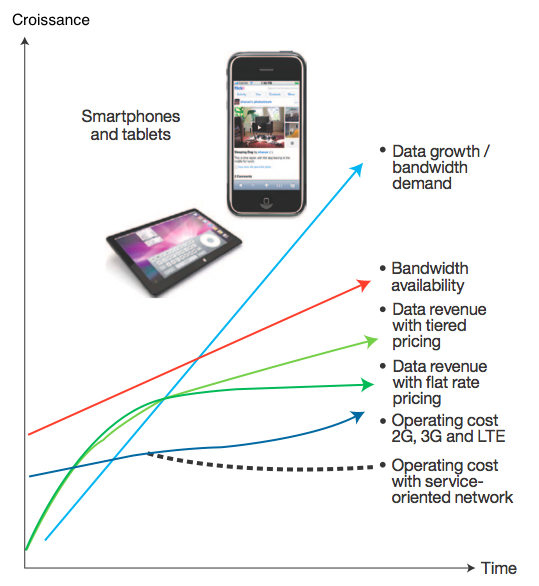
\includegraphics[width=15cm]{images/IncreasingPressureOnNetworkInfra.png} %ou image.png, .jpeg etc.
\caption{ Pression croissante sur l'infrastructure réseau \cite{IBMManagingGrowingPainsNeed}} %la légende
\label{image_soleil} %l'étiquette pour faire référence à cette image
\end{figure} %on ferme l'environnement figure


% Figure 1: The need for network capabilities and bandwidth is expanding at a faster rate than either bandwidth availability or revenue to grow

\clearpage

Le plus une entreprise dépend d'un nombre croissant de dispositifs et gros volumes de données, les plus importante est la demande pour débit et expansion de l'infrastructure. La complexité de cette expansion des réseaux augmente la probabilité des interruptions de service dues à une faille humaine ou autre problème. Ce fait met en évidence l'importance de la disponibilité, fiabilité, performance et sécurité. L'efficacité et la réduction des coûts deviennent cruciales pour aboutir la mis en échelle de ces besoins, et donc le management assume en rôle primordial dans ce contexte. \cite{IBMManagingGrowingPainsNeed}
 

Malgré l'assistance des agents autonomes et intelligents ainsi que des logiciels pour le management réseau, la mission de l'administrateur réseau reste importante et compliquée. Il doit équilibrer les différentes tâches du management pour assurer que le \gls{si} soit proprement configuré et maintenu. \cite{CentralIssuesNetworkManagementConclusion}

La configuration et l'installation du réseau exigent des techniciens experts hautement qualifiés sur plusieurs éléments le composant. Les interactions entre les nœuds du réseau (switches, routeurs etc.) sont complexes, ce qui provoque le besoin pour une approche système englobant la simulation. Avec l'interface de programmation courante des équipements réseau d'aujourd'hui, cela est difficile d'atteindre. De plus, les coûts opérationnels impliqués à l'approvisionnement et management de réseaux larges et multi-vendeurs  couvrant plusieurs technologies ont augmenté récemment, alors que les revenues se diminuent. \cite{ImplementationChallengesForSDN}

L'architecture réseau n'a pas été conçue pour le management, pourtant les administrateurs des réseaux d'aujourd'hui rencontrent des problèmes critiques de configuration, ingénierie du trafic, politique de routage et diagnostic de failles. Leurs outils pour analyse du trafic sont faibles et leurs mécanismes pour contrôler les opérations réseau ne facilitent pas la prédictibilité entre les relations de cause-effet. On réalise que l'opération et le management du réseau représentent la source la plus importante des coûts opérationnels, de failles et d'interruptions à cause d'erreurs des opérateurs. Un changement dans ce domaine est requis pour le design de l'architecture. \cite{NGSIManagement}

%Yet at the same time, society is daring the Internet to face the following set of challenges:
%Security: The lack of security in the Internet is worrisome to ev- eryone including users, application developers, and network and service operators.
%Mobility: Currently, application developers find little support for new mobile applications and services.
%Reliabilityandavailability: ISPsfacethetaskofprovidingaser- vice which meets user expectations of the Internet’s crucial role in both business and private life, in terms of reliability, resilience, and availability, when compared, for example, to the telephone network (five nines1). Furthermore, the service has to be seamless.
%Problem analysis: The toolset for debugging the Internet is lim- ited, e. g., tools for root cause analysis.
%Scalability: Questions remain regarding the scalability of some parts of the current Internet architecture, e.g., the routing system.
%Quality of Service: It is still unclear how and where to integrate different levels of quality of service into the architecture.
%Economics: Besides these more technical questions, there is also the question of how network and service operators can con- tinue to make a profit.



%A new network model is required to support this.
\section{Un nouveau modèle réseau pour supporter ces évolutions}
%\section{Clean-slate Internet}

%While the overall architecture is an undeniable success, the state of the networking industry and the nature of networking infrastructure is a less inspiring story. It is widely agreed that current networks are too expensive, too complicated to manage, too prone to vendor-lockin, and too hard to change. Moreover, this unfortunate state-of-affairs has remained true for well over a decade. Thus, while much of the research community has been focusing on “clean-slate” designs of the overall Internet architecture, a more pressing set of problems remain in the design of the underlying network infrastructure. That is, in addition to worrying about the global Internet protocols, the research community should also devote effort to how one could improve the infrastructure over which these protocols are deployed.

Même si globalement l'architecture réseau d'internet est un succès incontestable, l'état de l'industrie réseau et l'essence de son infrastructure est moins inspirant. Il est partout accepté que les réseaux courants sont excessivement chers, compliqués à gérer, sujets aux blocages des fournisseurs et difficiles à évoluer. En plus, cette condition a bien durée plus d'une décade. \cite{fabricIntro}



En résumé, l'infrastructure réseau confronte actuellement ces challenges:
\begin{itemize}
\item Sécurité : la manque de sécurité est assez inquiétante à tout niveau : des utilisateurs, aux développeurs aux opérateurs de services.
\item Mobilité : il existe très peu de support aux applications et services mobiles
\item Fiabilité et disponibilité : le nouvel usage de l'internet exige de plus en plus haute fiabilité et disponibilité.
\item Analyse de problèmes : les outils pour déboguer les failles réseau sont assez limités.
\item Évolution : certaine partis de l'architecture courante semblent être saturés, comme le système de routage.
\item Qualité de service : il est toujours incertain comment intégrer différents niveaux de qualité de service.
\item Économique : en outre de tous questions techniques, il reste aussi la question de comment les opérateurs pourront continuer à tirer profit.
\end{itemize}
\cite{InernetCleanSlateDesignIntro}

%In the past 30 years the Internet has been very successful using an incremental approach. However due to its success, the commu- nity has now reached a point where people are unwilling or unable to experiment on the current architecture. Therefore, it might be time to explore a clean-slate approach
Dans les dernières 30 années, internet a été bien succédé à utiliser une approche incrémentielle pour répondre aux divers challenges rencontrés. Cependant, grâce à ce succès, la communauté a récemment atteint un point où les personnes sont peu disposées ou incapables d'expérimenter sur cette architecture.  Pour cette raison, il est peut être le moment de d'explorer une nouvelle approche. \cite{InernetCleanSlateDesignApproach}

%Re-partir de zéro. En le faisant, quels sont les caractéristique de l'architecture ?


Cette problématique a amené scientistes et les ingénieurs impliqués à concevoir \gls{sdn}. \gls{sdn} est un nouveau \glslink{paradigme}{paradigme} réseau qu'on fait actuellement en cours de développer pour adapter l'infrastructure existante au nouveau scénario.


%\section{Les requis d'un réseau idéalement adapté aux besoins courants}
\chapter{Réseaux programmables avec SDN}

On cherche à concevoir une architecture plus adaptée aux enjeux de la communication de l'actualité discutés dans le chapitre 1. Cette problématique a amené scientistes et les ingénieurs impliqués à concevoir \gls{sdn}. \gls{sdn} est un nouveau \glslink{paradigme}{paradigme} réseau qu'on est actuellement en cours de développer pour adapter l'infrastructure existante à ce nouveau scénario.
Le but de ce chapitre est de (re)définir SDN et de présenter en quoi SDN répond aux besoins explicités dans le chapitre 1.
%Ce chapitre répond aux questions : Qu'est-ce que SDN ? Qu'est-ce que cela propose ?
Le chapitre propose aussi un point sur la situation de SDN, en présentant les organisations qui l'adopte et ce qui a été développé en terme de standards et protocoles.

\section{Séparation de l'intelligence (contrôle) de la commutation (flux de données)}

%Having recognized the problem, the networking commu- nity is hard at work developing programmable networks, such as GENI [1] a proposed nationwide research facility for experimenting with new network architectures and dis- tributed systems. These programmable networks call for programmable switches and routers that (using virtualiza- tion) can process packets for multiple isolated experimen- tal networks simultaneously.
Ayant adressé cette problématique, la communauté réseau fait beaucoup d'efforts pour le développement des réseaux programmables. Ces réseaux programmables utilisent des switches et des routeurs programmables qui peuvent traiter des paquets pour des multiples réseaux expérimentaux  à la fois, grâce à la \gls{virtualisation}. \cite{OpenFlowStanfordOssification} Divers projets pour les réseaux programmables, comme NETCONF \cite{NETCONF}, Ethane \cite{Ethane}, GENI \cite{GENI} etc. ont été réalisés et en ont servi de base pour ce paradigme qu'on développe et supporte aujourd'hui : \gls{sdn}. 

%SDN is described in this article with the Open Networking Foundation (ONF) [1] definition: “In the SDN architecture, the control and data planes are decoupled, network intelli- gence and state are logically centralized, and the underlying network infrastructure is abstracted from the applications.”

SDN est défini au long de cette étude  selon \gls{onf} : Dans l'architecture SDN, les plans de contrôle et de données sont découpés, l'intelligence et l'état du réseau sont logiquement centralisés, et l'infrastructure du réseau est donc abstraite des applications. \cite{SDNNewNormONFExecutiveSummary}


%The control plane is responsible for configuration of the node and programming the paths that will be used for data flows. Once these paths have been determined they are pushed down to the data plane. Data forwarding at the hardware level is based on this control information.

Le \gls{controlplane} est responsable pour la configuration d'un nœud et pour la programmation des chemins qui seront utilisés par les flux de données. Le \gls{dataplane} fourni au hardware les informations nécessaires à la commutation. \cite{ImplementationChallengesForSDNBackground}



Dans l'architecture réseau traditionnellement déployée, chaque équipement actif contient un plan de contrôle et un plan de données à l'intérieur du même matériel. L'ossification d'internet discuté dans le chapitre 1 est largement attribuée à ce fort couplage entre les deux plans provocant que toutes les décisions sur les flux de donnés soient embarquées dans chaque élément réseau. La manque d'une interface de contrôle commune à tous les dispositifs complique toute évolution que cela soit un simple changement de configuration ou le développement d'une nouvelle application. \cite{SurveySDNArchi}



%As mentioned previously, the so-called Internet “ossifica- tion” [2] is largely attributed to the tight coupling between the data– and control planes which means that decisions about data flowing through the network are made on-board each network element. In this type of environment, the deployment of new network applications or functionality is decidedly non- trivial, as they would need to be implemented directly into the infrastructure. Even straightforward tasks such as config- uration or policy enforcement may require a good amount of effort due to the lack of a common control interface to the various network devices.

Avec SDN, on propose la séparation de ces deux éléments. Le \gls{controlplane} est implémenté par un contrôleur centralisé est commun à tous les équipements qui passent à contenir seulement le \glspl{dataplane} un plus d'un module de communication.  La séparation de la fonction de commutation de la logique de contrôle permet un déploiement plus facile de nouveaux protocoles et applications. La virtualisation et le management du réseau deviennent plus simples et les nombreux \glspl{middlebox} sont consolidés dans le logiciel de contrôle. \cite{SurveySDNArchi} \cite{SDNNewNormONFExecutiveSummary}
%the separation of the forwarding hardware from the control logic allows easier deployment of new protocols and applications, straightforward network visualization and management, and consolidation of various middleboxes into software control.

Dans l'image ci-dessous on voit un schéma illustrant l'ensemble de l'architecture dans les deux cas.

%\begin{figure}[!h] %on ouvre l'environnement figure
%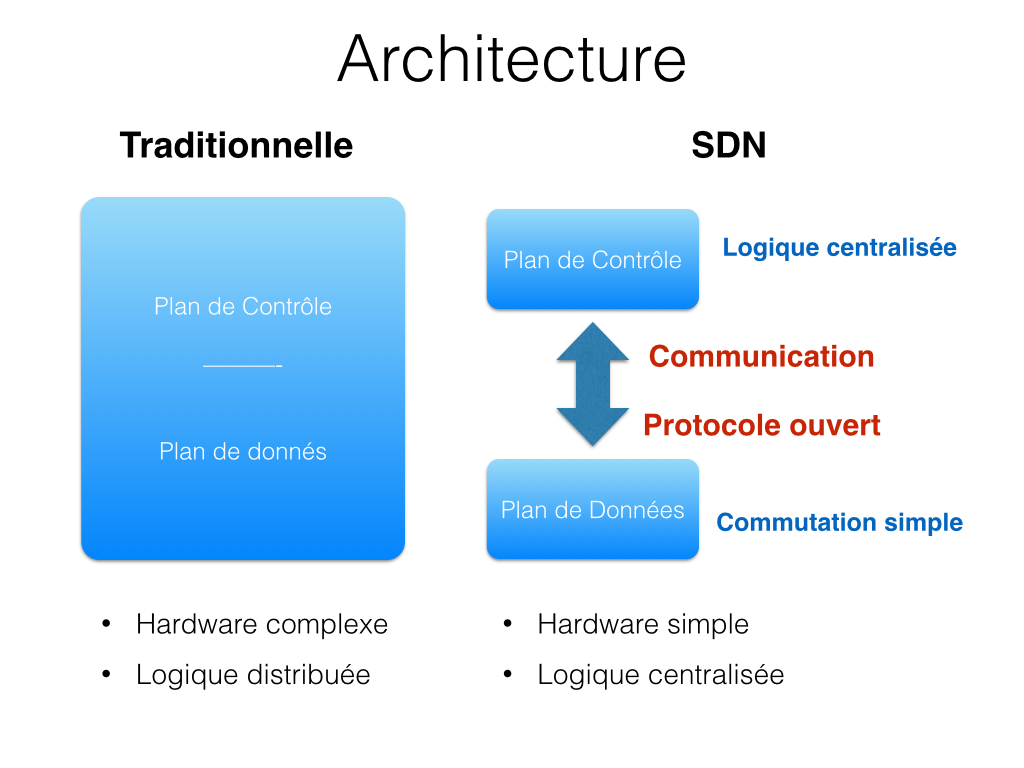
\includegraphics[width=15cm]{images/ComparaisonArchis.png} %ou image.png, .jpeg etc.
%\caption{ Un équipement actif dans l'Architecture Traditionnelle et SDN} %la légende
%\label{imgNodesArchi} %l'étiquette pour faire référence à cette image
%\end{figure} %on ferme l'environnement figure



\begin{figure}[!h] %on ouvre l'environnement figure
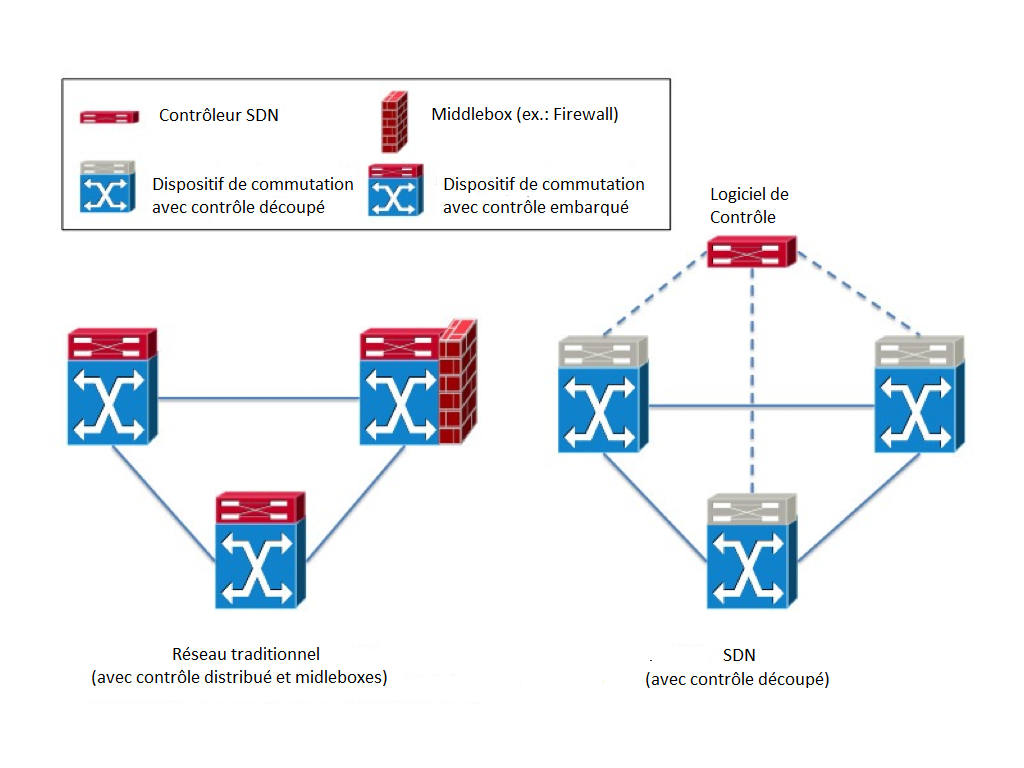
\includegraphics[width=15cm]{images/TraditionalVsSDN.png} %ou image.png, .jpeg etc.
\caption{ L'ensemble de l'Architecture Traditionnelle et SDN \cite{SurveySDNArchi}} %la légende
\label{imgOverviewArchi} %l'étiquette pour faire référence à cette image
\end{figure} %on ferme l'environnement figure

Avec l'approche \gls{sdn} les switchees sont contrôles par un \gls{nos} qui fourni un modèle abstrait de la topologie du réseau au contrôleur \gls{sdn} hébergeant les applications. Le contrôleur peut donc exploiter cet vue globale du réseau pour optimiser le management des flux et supporter les requis de 'scalabilité' et de flexibilité.

%From these service-focussed requirements, SDN has emerged. Control is moved out of the individual network nodes and into the separate, centralized controller. SDN switches are con- trolled by a Network Operating System (NOS) that collects information using the API shown in Figure 2B and manipulates their forwarding plane, providing an abstract model of the network topology to the SDN controller hosting the applications.

\clearpage



\section{Un point sur la situation}
%\subsection{ONF}

%The Open Networking Foundation (ONF) is a non‑profit, user‑driven organization dedicated to accelerating the adoption of open Software‑Defined Networking (SDN). We view SDN as a disruptive approach to networking that will change how virtually every company with a network operates.

%Launched in 2011 by Deutsche Telekom, Facebook, Google, Microsoft, Verizon, and Yahoo!, ONF is a nonprofit organization dedicated to rethinking networking, and quickly and collaboratively bringing to market SDN standards and solutions. ONF is accelerating the delivery and commercialization of SDN and fostering a vibrant market of products, services, applications, customers, and users. 


Open Networking Foudation (\gls{onf}) et une organisation non-profit et axée sur l'utilisateur dédiée à l'accélération de l'adoption ouverte de SDN. Cette organisation voit SDN comme une approche réseau qui va changer comment opère chaque entreprise avec un réseau.
\gls{onf} a été initiée en 2011 par Deutsche Telekom, Facebook, Google, Microsoft, Verizon et Yahoo! dans le but de repenser en collaboration les réseaux informatiques et rapidement apporter au marché les solutions et les standards SDN. Avec la collaboration de  grands experts mondiaux, ONF accélère la commercialisation de SDN en favorisant un vif marché de produits, services, applications, clients et utilisateurs. ONF compte aujourd'hui avec plus de 100 entreprises membres collaboratives de tout taille et variété. \cite{ONFOverview}

\gls{onf} a fait des efforts de standardiser le protocole \gls{openflow}. Ce protocole focalise en standardiser les interfaces entre les applications et le contrôleur et les interfaces entre le contrôleur et l'équipement de commutation.\cite{SurveySDNArchi}
%The Open Network Foundation (ONF) [3] has been trying to standardize the OpenFlow protocol. As the control plane abstracts network applications from underlying hardware infrastructure, they focus on standardizing the inter- faces between: (1) network applications and the controller (i.e. northbound interface) and (2) the controller and the switching infrastructure (i.e., southbound interface) which defines the OpenFlow protocol itself. 

Le fort support de l'industrie, de la recherche et des académies que \gls{onf} et la proposition de \gls{sdn} ont pu recueillir est assez expressif. Les résultats dans ces différents secteurs ont produit un nombre significatif de livrables dans la forme d'articles de recherche, d'implémentations de logiciels de référence et même de hardware. Il y a eu également des efforts de standardisation de SDN de la part d'autres organisations produisant des normes, comme IETF et IRTF. \cite{SurveySDNIntro}
%The strong support from industry, research, and academia that the Open Networking Foundation (ONF) and its SDN proposal, OpenFlow, has been able to gather is quite impres- sive. The resulting critical mass from these different sectors has produced a significant number of deliverables in the form of research papers, reference software implementations, and even hardware. So much so that some argue that OpenFlow’s SDN architecture is the current SDN de-facto standard. In line with this trend, the remainder of this section focuses on OpenFlow’s SDN model. 

%On the academic side, the OpenFlow Network Research Center [4] has been created with a focus on SDN research. There have also been standardization efforts on SDN at the IETF and IRTF and other standards producing organizations.


%\subsection{OpenFlow - Protocoles standardisés}
%\section{Dispositifs de commutation}
%The basic idea is simple: we exploit the fact that most modern Ethernet switches and routers contain flow-tables (typically built from TCAMs) that run at line-rate to im- plement firewalls, NAT, QoS, and to collect statistics. While each vendor’s flow-table is different, we’ve identified an in- teresting common set of functions that run in many switches and routers. OpenFlow exploits this common set of func- tions.

SDN profite du fait que la majorité des switches et routeurs existants contiennent des tableaux de flux qui exécutent à une fréquence ligne pour implémenter leurs protocoles et collecter des statistiques.



%\section{Contrôleur}
Controllers. A controller adds and removes flow-entries from the Flow Table on behalf of experiments. For example, a static controller might be a simple application running on a PC to statically establish flows to interconnect a set of test computers for the duration of an experiment. In this case the flows resemble VLANs in current networks— providing a simple mechanism to isolate experimental traffic from the production network. Viewed this way, OpenFlow is a generalization of VLANs.


\chapter{Enjeux de SDN}

Ce chapitre présente quels sont les enjeux pour déployer SDN. Il a pour but d'identifier les challenges lors de la mise en place de cette architecture ainsi que les problèmes susceptibles d'être rencontrés. Pour chaque enjeux, les idées pour les surmonter sont montrées tout en proposant les compromis de ces solutions.

\section{Contrôle : centralisé ou distribué}
Contrôle centralisé = un seul point de faille pour le réseau complet.

Architecture physiquement distribuée mais centralisé au niveau logique.

Consistence et stateliness quand on distribue des états sur le réseau peut causer un mal comportement des applications qui pensent qu'elles une vision précise du réseau.

\section{Niveau de granularité}

\section{Politiques : réactives ou pro-actives}

\section{Fonctions de Virtualisation du Réseau}
%\gls{nfv}

\chapter{Possibilités d'Application de SDN}

%Ce chapitre a pour but de présenter ce qui apporte SDN, quelles sont les applications pratiques de ce nouvel paradigme. Ce ne sera pas exhaustive, mais c'est pour exemplifier. Cela permettra aussi d'avoir une idée de l'exploitation future de SDN.

Une infinité d'applications et de cas d'utilisations sont imaginables. Ce chapitre propose d'analyser les enjeux auxquels on espère pouvoir répondre avec SDN et de présenter des applications ciblées sur ces attentes. De cette analyse, les cas d'utilisation plus cohérents seront identifiés et ensuite détaillés.

 
%\section{Identifications des applications espérées par les utilisateurs}

%In August and September of 2013 a survey was given to the subscribers of Webtorials.
Entre les mois d'août et septembre de 2013, Webtorials a réalisé un sondage auprès de ses abonnés. Une des enquêtes a été sur les challenges et opportunités qu'ils pensent pouvoir résoudre avec SDN au sein des entreprises de \gls{ti} typiques. Le tableau 3.1 affiche le pourcentage de réponses positives pour chaque challenge. \cite{2013GuideSDNNVUseCases}

\begin{table}[!h]
\centering
\begin{tabular}{|p{12cm}|c|}
\hline 
\bf Challenge ou Opportunité & \bf Pourcentage \\ 
\hline 
Meilleure utilisation des ressources réseau & 51\% \\ 
\hline 
Simplifier la configuration de la QoS et de la sécurité  & 47\%  \\
\hline 
Réaliser l'ingénierie du trafic avec vision point-à-point du réseau & 44\% \\ 
\hline 
Évolution plus facile des fonctions réseau & 39\% \\ 
\hline 
Support dynamique de la gestion de ressources virtuelles  & 38\% \\ 
\hline 
Établissement des réseaux Ethernet virtuels sans les contraintes de configuration des VLANs & 35\% \\ 
\hline 
Réduction de la complexité & 34\% \\ 
\hline 
Permettre les demandes dynamiques de services au réseau & 32\% \\ 
\hline 
Réduction des dépenses d'exploitation & 30\% \\ 
\hline 
Faire évoluer les fonctionnalités réseau plus rapidement en s'appuyant sur les cycles de vie du développement logiciel & 27\% \\ 
\hline 
Implémentation plus facile de la QoS & 27\% \\ 
\hline 
Implémentation des fonctionnalités de sécurité plus efficaces & 26\% \\ 
\hline 
Réduction des dépenses d'investissement de capital & 25\% \\ 
\hline 
Absence de challenges/opportunités pouvant être adressés par SDN & 3\% \\ 
\hline 
\end{tabular}
\caption{Opportunités et Challenges pouvant être résolus par SDN \cite{2013GuideSDNNVTable11}}
\end{table} 

\clearpage

Les réponses sont en accord avec d'autres enquêtes, comme celle dirigée par Heavy Reading, où 27 dirigeants seniors ont été interviewés    sur les éléments clés de déploiement. \cite{SDNNFVWAN} De ces résultats on peut conclure que le marché compte pouvoir bénéficier de SDN sur une vaste gamme de défis et opportunités, ce qui démontre des attentes tout à fait favorables pour cette technologie. Cette variété de sujets est en général intéressante pour l'adoption du \gls{paradigme} mais peut causer des confusions au début, en ralentissant les actions à ce moment-là.

Dans le sondage fait par Webtorials, d'autres questions ont été posées. Par exemple, les participants ont répondu que si leurs sociétés implémentaient SDN dans les deux ans qui suivent, ce serait plus probable que ce soit sur : \gls{datacenter} (54\%), réseau d'entreprise et/ou campus (26\%), WAN (23\%) ou pas d'implémentation SDN (11\%) \cite{2013GuideSDNNVTable12}. Par conséquent, les applications présentées ci-après sont classées en fonction de ces trois cibles de déploiement.




\section{Data Center}



%Most networking vendors offer data center fabric solutions featuring some form of Layer 2 multi-pathing to improve the networks capacity to handle “east-west” traffic flow characteristic of server virtualization, converged storage networking, and cluster computing. SDN provides an effective solution to this problem because the network path is determined by a central controller and does not require the use of STP. Thus, all inter-switch links can be fully utilized and traffic can be directed between multiple LANs without the need for first routing the traffic to higher-level switches.



\textbf{\glspl{vlan}} :

SDN peut facilement fournir aux utilisateurs leurs propres réseaux isolés, comme les VLANs. L'approche la plus simple est de déclarer statiquement les ensembles de flux qui spécifient les ports accessibles par un VLAN ID donné. Le trafic identifié venant d'un type d'utilisateur (à l'origine d'un port du switch ou d'une adresse MAC spécifiés) est marqué dans le VLAN ID approprié. Une approche plus dynamique pourrait utiliser le contrôleur pour gérer l'authentification des utilisateurs et utiliser les informations sur leur localisation pour marquer le trafic à la volée. \cite{OpenFlowStanfordUsing} 

%VLANs. OpenFlow can easily provide users with their own isolated network, just as VLANs do. The simplest approach is to statically declare a set of flows which specify the ports accessible by traffic on a given VLAN ID. Traffic identified as coming from a single user (for example, originating from specific switch ports or MAC addresses) is tagged by the switches (via an action) with the appropriate VLAN ID. A more dynamic approach might use a controller to manage authentication of users and use the knowledge of the users’ locations for tagging traffic at runtime.



\textbf{Répartition de charge et sécurité} : 

FlowScale est une application basée sur OpenFlow qui fournit la répartition de charge du trafic réseau en utilisant le switch OpenFlow. L'application a été utilisée dans un système \gls{ids} pour distribuer uniformément le trafic  aux capteurs. Lorsqu'il sera complètement déployé, le système sera capable de distribuer le trafic à de taux dépassant 500Gb/s.  \cite{FlowScale}
%Indiana University has developed an OpenFlow-based, load-balancing application called FlowScale. According to the University 15, “FlowScale provides complex, distributed load balancing of network traffic using an OpenFlow-capable Top of Rack (ToR) switch. IU deployed the application into its Intrusion Detection System (IDS) to distribute traffic evenly to sensors. When fully deployed, the system will span the IU Bloomington and IUPUI networks and have the capability to distribute traffic at rates exceeding 500Gb/s.”

%\bf{Monitoring Réseau}. Avec SDN, la redirection de flux réseau peut être programmée, permettant de surveiller le trafic sélectionne sans le rediriger physiquement.  
%Network Taps. With OpenFlow virtual ports, the functionality of a network tap can be programmed into the OpenFlow switch, allowing selected traffic to be monitored without deploying physical taps. Traffic can also be replicated and redirected to any monitoring device in the network. Big Switch networks has announced such a network monitoring application referred to as Big Tap 16.



\textbf{Economie d'énergie} : 

ElasticTree est un gestionnaire d'énergie pour le réseau. Le projet utilise SDN pour trouver la configuration la réseau plus économique qui satisfera les conditions de trafic en éteignant les équipements qui ne sont pas nécessaires. Le projet a obtenu des économies d'énergie entre 25 et 62\% sous diverses conditions de trafic \cite{Elastictree}. Ces économies peuvent être augmentées en introduisant la virtualisation et la gestion des serveurs. Une possibilité est le travail Honeyguide qui propose une optimisation d'énergie en utilisant la migration de \glspl{vm} pour augmenter la quantité de \glspl{vm} et de switches pouvant être arrêtés \cite{Honeyguide}.


%They proposed ElasticTree, a network-wide power manager that utilizes SDN to find the minimum-power network subset which satisfies current traffic conditions and turns off switches that are not needed. As a result, they show energy savings between 25-62\% under varying traffic conditions. One can imagine that these savings can be further increased if used in parallel with server management and virtualization; one possibility is the Honeyguide[80] approach to energy optimization which uses virtual machine migration to increase the number of machines and switches that can be shutdown.


\textbf{Applications sur Cloud Computig} : 

Dans les offres \gls{iaas}, les utilisateurs ont une vision et un contrôle du réseau  limités. Les technologies SDN peuvent faciliter la délégation du contrôle du réseau et fournir certains niveaux d'abstraction aux utilisateur finaux, leur permettant de configurer leur partie de réseau. De plus, les offres \gls{cloudcomputing} basées sur SDN pourront fournir des services de bande passante sous demande, avec un approvisionnement automatisé et intelligent, dirigés par une logique d'orchestration cloud et par les besoins des clients. \cite{AdoptionResearchTrendsCloud}

%Offering Infrastructure as a Service (IaaS), users only get a logical view of the underlying network and have limited control. SDN technologies have the capabilities to facilitate delegation of network controls and provide some level of network abstractions to end-users to enable them to configure their slice of the network. Delegating more control to the end-users could raise security concerns for the providers [Azodolmolky13]. SDN-based clouds will allow enterprises to have multi-vendor networks to avoid vendor lock-in. They can access dynamic bandwidth for ad- hoc, timely inter-data center workload migration and processing; and eliminate the burden of underutilized, costly high-capacity fixed private leased lines. SDN-enabled bandwidth-on-demand services provide automated and intelligent service provisioning, driven by cloud service orchestration logic and customer requirements.



\textbf{Raccordement réseau de deux data centers} : 

SDN permet de relier des réseaux au niveau de la couche 2 à travers de multiples data centers, les connectant comme s'ils étaient dans un seul réseau. Avec cette fonctionnalité, les architectes d'applications peuvent par exemple placer leurs "compute clusters" plus près de leur point d'usage et supporter une récupération efficace après incident. \cite{ODCAusageScenarios} L'image \ref{imgDCL2B} illustre ce raccordement.
%Data Center L2 Network Bridging. SDN enables bridging of Layer 2 networks across multiple data centers, providing a single overlay network. With this capability, application architects can place compute clusters closer to their point of usage and support effective disaster recovery.

\begin{figure}[!h] %on ouvre l'environnement figure
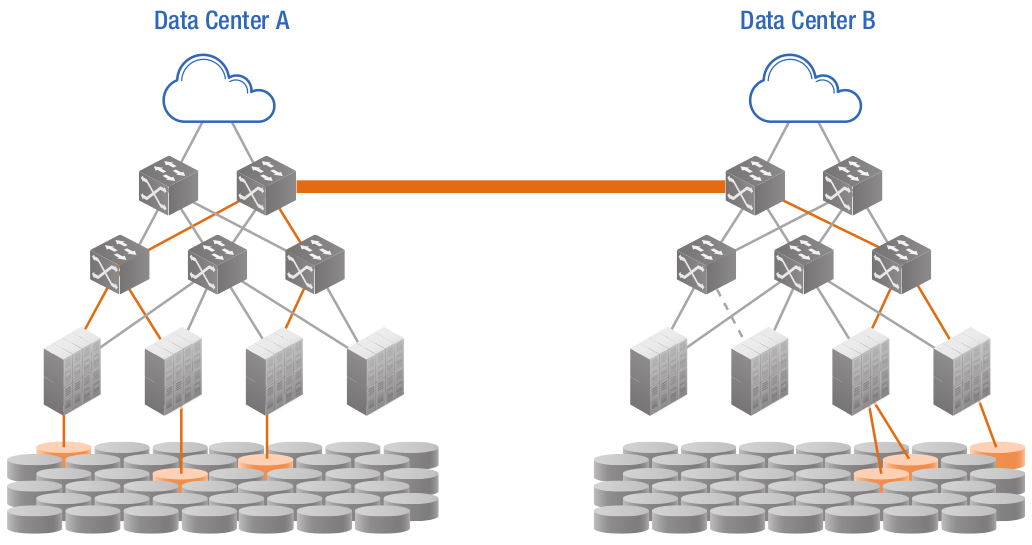
\includegraphics[width=15cm]{images/DataCenterL2Bridging.png} %ou image.png, .jpeg etc.
\caption{ Raccordement réseau de deux Data Centers \cite{ODCAusageScenarios}} %la légende
\label{imgDCL2B} %l'étiquette pour faire référence à cette image
\end{figure} %on ferme l'environnement figure

Les applications sur l'automatisation de services réseaux dans les data centers sont les plus attendues. Par conséquent,  elles seront les plus représentées sur le marché, ce qu'il sera développé dans le prochain chapitre.


\section{Réseaux d'entreprise et campus}

Souvent les entreprises qui gère des grands réseaux ont des pré-requis stricts en terme de performance et sécurité, qui peuvent largement varier selon divers facteurs. Par exemple, les réseaux des universités sont considérés comme un cas spécial de réseaux d'entreprises : dans cet environnement, plusieurs dispositifs connectés sont temporaires et ne sont pas contrôlés par l'institution, mettant en outre en question la sécurité et l'allocation de ressources. L'adéquation de la gestion est critique dans ces conditions et SDN peut être utilisé pour imposer et ajuster les politiques réseaux par programmation et ainsi aider à surveiller l'activité et réguler la performance.

%Enterprises often run large networks, while also having strict security and performance requirements. Furthermore, different enterprise environments can have very different requirements, characteristics, and user population, For example, University networks can be considered a special case of enterprise networks: in such an environment, many of the connecting devices are temporary and not controlled by the University, further challenging security and resource allocation. Additionally, Universities must often provide support for research testbeds and experimental protocols. Adequate management is critically important in Enterprise environments, and SDN can be used to programmatically enforce and adjust network policies as well as help monitor network activity and tune network performance.

\textbf{Management du réseau et contrôle d'accès} : 

%Une implémentation d'un contrôleur, adaptée pour le management et contrôle du réseau, qui gère l'admission et le routage des flux. 
L'idée de base est de permettre aux administrateurs réseaux de définir des politiques applicables à tout le réseau dans un contrôleur central. Ces politiques seront renforcées directement par la réalisation du contrôle d'admission sur le traitement de chaque nouveau flux. Le contrôleur vérifie que les flux soient en conformité avec un ensemble de règles, telles que "les hôtes peuvent communiquer via \glslink{http}{HTTP} seulement en passant par un proxy" ou "les téléphones VoIP ne sont pas autorisés à communiquer avec les laptops". Un contrôleur associe des paquets avec leurs émetteurs via la liaison entre noms et adresses. En résumé, il prend le contrôle du \gls{dns} et du \gls{dhcp} et authentifie tous les utilisateurs qui se rejoignent, gardant trace des ports de switches ou point d'accès utilisés pour la connexion.

%Network Management and Access Control. An implementation of a controller, suited for network management and control, that manages the admittance and routing of flows. The basic idea is to allow network managers to define a Controller network-wide policy in the central controller, which is enforced directly by making admission control decisions for each new flow. A controller checks a new flow against a set of rules, such as “Guests can communicate using HTTP, but only via a web proxy” or “VoIP phones are not allowed to communicate with laptops.” A controller associates packets with their senders by managing all the bindings between names and addresses — it essentially takes over DNS, DHCP and authenticates all users when they join, keeping track of which switch port (or access point) they are connected to. \cite{OpenFlowStanfordUsing}


\textbf{Connexion sans fils mobile}.

Plusieurs tentatives ont été focalisés dans la connectivité omniprésente dans le contexte des infrastructures basées sur l'accès sans fil au réseau, comme le WiFi. Par exemple, des expériences ont été faites pour les clients mobiles VoIP sur la proposition d'un nouveau mécanisme de transfert d'appel. Un contrôleur est implémenté pour tracer la localisation des clients et être capable de re-router les connexions (avec la re-programmation des tables de flux) au moment où les utilisateurs se déplacent dans le réseau. Cela permettra le transfert transparent d'un point d'accès à l'autre sans coupure de l'appel. \cite{OpenFlowStanfordUsing}

%Infrastructure-based Wireless Access Networks. Several efforts have focused on ubiquitous connectivity in the context of infrastructure-based wireless access networks,such as cellular and WiFi.
%Mobile wireless VOIP clients. For this example consider an experiment of a new call-handoff mechanism for WiFi-enabled phones. In the experiment VOIP clients establish a new connection over the OpenFlow-enabled network. A controller is implemented to track the location of clients, re-routing connections — by reprogram-ming the Flow Tables — as users move through the network, allowing seamless handoff from one access point to another. \cite{OpenFlowStanfordUsing}



Le protocole OpenFlow, généralement admis comme standard SDN et introduit dans le chapitre suivant, a été proposé en 2008 par Stanford (US) pour résoudre la problématique particulière de l'innovation sur les réseaux de campus. La flexibilité recherchée a été telle que le résultat des travaux n'ont pas seulement répondu à ce point précis, mais SDN s'est montré aussi intéressant dans d'autre domaine d'activités citées dans ce chapitre. \cite{OpenFlowStanfordOssification}


\section{WAN}
Dans un \gls{wan}, la centralisation permet le calcul déterministe et optimal de routes pour chaque flux avec l'utilisation d'un modèle complet de la topologie de bout-en-bout du réseau. L'allocation de bande passante peut être contrôlée dynamiquement à la demande lors des changements de trafic. Le résultat peut être une meilleure utilisation du réseau sans sacrifier la qualité de service. Le traitement centralisé de route permet aussi de pré-déterminer les routes alternatives pour chaque lien en cas de panne. On peut profiter de la puissance de traitement des processeurs à multiples cœurs et/ou des \glspl{cluster} pour le calcul de routes et le traitement des flux. Cette application correspond à une de trois opportunités les plus attendues d'après le sondage. \cite{2013GuideSDNNVUseCases}


%Centralization allows optimum routes to be calculated deterministically for each flow by leveraging a complete model of the end-to-end topology of the network. Bandwidth allocations can be controlled dynamically to provide bandwidth on demand with changing traffic patterns. The result can be much better utilization of the network without sacrificing service quality. Centralized route processing also allows the pre-computation of a set of fail-over routes for each possible link or node failure. Centralized processing also can take advantage of the virtually unlimited processing power of multi-core processors and cluster computing for calculating routes and processing new flows. As shown in Table 11, being able to do end-to-end traffic engineering is one of the top three opportunities that The Survey Respondents associate with SDN.



Avec SDN, le trafic WAN peut être aussi dynamiquement re-routé pour réduire/contrôler la latence des applications sensibles, comme la voix sur IP. La charge du trafic peut être également repartie sur des chemins parallèles à différents coûts.
%WAN traffic can be dynamically rerouted to reduce/control latency for VoIP and other latency sensitive applications. Traffic can also be load balanced over parallel paths of differing costs.
La mesure des flux en temps réel permettrait de limiter le débit ou de modifier la transmission pour optimiser la performance des applications. Par exemple, le contrôleur peut configurer un switch compatible pour modifier les marquage \gls{qos} afin de changer les priorités sur les chemins point-à-point restants.
%With OpenFlow V 1.3, per flow meters can be used for rate limiting or to provide real time visibility of application performance allowing the controller to modify forwarding behavior to maximize application performance. For example, the controller can configure an OpenFlow switch to modify the QoS markings to change the priority received over the remainder of the end-to-end path.
La récupération des liens échoués peut être atteinte avec la sélection dynamique de chemins, tenant compte des mesures de performance, des états de ports et des niveaux d'utilisations par les nœuds.
%With extensions in V1.3 and V1.4, OpenFlow can support circuit-switched paradigms, including CWDM, DWDM, and MPLS with specific path selection and requested levels of CBR and priority. Circuits can be provisioned on a dynamic, scheduled, or permanent basis. Recovery from failed circuits can be via predetermined backup paths or by dynamic path selection. Circuit provisioning can take into account performance metrics, port states, and endpoint utilization.

Un exemple pratique d'une application réelle de SDN a été présentée par Google. L'entreprise a présenté dans la conférence "Open Network Summit" \cite{googleONS} une implémentation à grande échelle d'un réseau SDN connectant des \glspl{datacenter} partout dans le monde. Le travail, intitulé B4 \cite{SDNWANB4}, présente en détails la conception, l'implémentation et l'évaluation de ce réseau connectant les \glspl{datacenter} Google géographiquement distribués. 
%L'image \ref{GoogleOpenFlowWAN} visualise le déploiement modial de B4. 
Le travail décrit un des premiers et plus grands déploiements SDN. Sa motivation a été le besoin pour des routes et l'ingénierie de trafic personnalisées ainsi que le haut niveau de \gls{scalability}, tolérance aux failles, rentabilité et contrôle requis et ne pouvant pas être accomplis avec l'architecture WAN traditionnelle. La solution a proposé une architecture SDN basée sur OpenFlow construite pour contrôler des switches particuliers. Après trois ans en production, B4 se montre efficace dans le sens qu'il dirige des nombreux liens avec une utilisation à près de 100\% et en même temps partageant les flux sur des multiples chemins. \cite{SurveySDNApplications}


\begin{figure}[!h] %on ouvre l'environnement figure
\centering
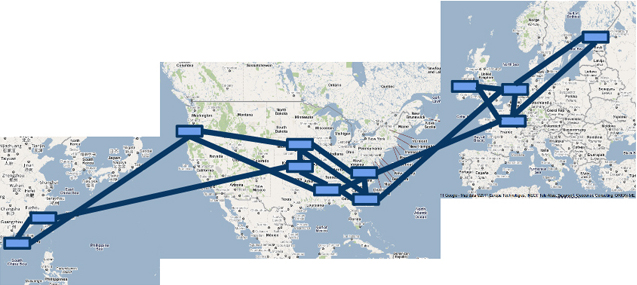
\includegraphics[width=13cm]{images/GoogleOpenFlowWAN.jpg} %ou image.png, .jpeg etc.
\caption{ Déploiement mondial de B4 en 2011 \cite{SDNWANB4}} %la légende
\label{GoogleOpenFlowWAN} %l'étiquette pour faire référence à cette image
\end{figure} %on ferme l'environnement figure



%Dans le cadre des réseaux WAN, les cas d'utilisations SDN se complètent avec ceux de \gls{nfv}. NFV, comme SDN, propose aussi une architecture réseau visant plutôt des opérateur/fournisseurs de services réseau. NFV a un rôle sur certaines applications SDN, et vice versa. \cite{SDNNFVWAN} L'approfondissement sur la problématique WAN pourrait donc être complété par un examen de l'architecture NFV, mais cet aspect ne sera pas traité dans cette étude.





%La description du concept de \gls{nfv}, qui propose aussi une architecture réseau, dépasse les délimitations de l'objet de cette étude. Néanmoins, il est à savoir que la solution a lieu plutôt chez les opérateur/fournisseurs de services réseau et que NFV a un rôle sur certaines applications SDN, et vice versa. L'approfondissement sur la problématique WAN pourrait donc être complémenté par un examen de l'architecture NFV, hors-sujet mais aussi intéressant.


%A practical example of a real application of the SDN concept and architecture in the context of data centers was presented by Google in early 2012. The company presented at the Open Network Summit [81] a large scale implementation of an SDN-based network connecting its data centers. The work in [82] presents in more detail the design, implementation, and evaluation of B4, a WAN connecting Google’s data centers world wide. This work describes one of the first and largest SDN deployments. The motivation was the need for customized routing and traffic engineering and the fact that the level of scalability, fault tolerance, cost efficiency and control required, could not be achieved by means of a traditional WAN architecture. A customized solution was proposed and an OpenFlow-based SDN architecture was built to control individual switches. After three years in production, B4 is shown to be efficient in the sense that it drives many links at near 100\% utilization while splitting flows among multiple paths. Furthermore, the experience reported in the work shows that the bottleneck resulting from control-plane to data-plane communication and overhead in hardware programming are important issues to be considered in future work. 



%\section{Management du Réseau et Contrôle d'Accès}
%Association des flux aux groupe d'utilisateur permettant de définir les politiques d'accès à différents services.

%\section{VLANs}
%Réseaux isolés définis par flux.

%\section{Clients mobiles sans fil VoIP}

Ces cas d'utilisations illustrent la variété de possibilités pouvant être réalisées avec SDN. Le prochain chapitre présente les offres du marché qui doivent donner les moyens de déployer ces applications.


\chapter{Solutions SDN disponibles}

Le but de ce chapitre n'est pas de détailler chaque solution SDN émergente, mais d'analyser les offres des principaux constructeurs du marché et leur positionnement par rapport aux tendances observées.
Tout d'abord un point sur la situation de SDN sera présentera, comment les entreprises supportant SDN se sont positionnées pour le développement de standards et de protocoles.



%https://www.opennetworking.org/sdn-resources/onf-products-listing

\section{Un point sur la situation}
%\subsection{ONF}

%The Open Networking Foundation (ONF) is a non‑profit, user‑driven organization dedicated to accelerating the adoption of open Software‑Defined Networking (SDN). We view SDN as a disruptive approach to networking that will change how virtually every company with a network operates.

%Launched in 2011 by Deutsche Telekom, Facebook, Google, Microsoft, Verizon, and Yahoo!, ONF is a nonprofit organization dedicated to rethinking networking, and quickly and collaboratively bringing to market SDN standards and solutions. ONF is accelerating the delivery and commercialization of SDN and fostering a vibrant market of products, services, applications, customers, and users. 


Open Networking Foudation (\gls{onf}) est une organisation non lucrative et axée sur l'utilisateur, dédiée à l'accélération de l'adoption ouverte de SDN. Cette organisation voit SDN comme une approche réseau qui va changer la façon dont chaque entreprise opère un réseau.
\gls{onf} a été initiée en 2011 par Deutsche Telekom, Facebook, Google, Microsoft, Verizon et Yahoo dans le but de travailler en collaboration pour repenser les réseaux informatiques et apporter rapidement au marché les solutions et les standards SDN. Avec la coopération de grands experts mondiaux, ONF accélère la commercialisation de SDN en favorisant un  marché dynamique de produits, de services, d'applications, de clients et d'utilisateurs. ONF compte aujourd'hui plus de 100 entreprises membres collaboratives, de toute taille et variété. \cite{ONFOverview}

\gls{onf} s'est fortement impliqué pour standardiser le protocole \gls{openflow}. Ce protocole se focalise sur la standardisation des interfaces entre les applications et le contrôleur et les interfaces entre le contrôleur et l'équipement de commutation. De grands noms de l'industrie (comme Cisco, Microsoft, Google etc.) ont réalisé des produits supportant OpenFlow, comme des switches. \cite{SurveySDNArchi} %Dans l'image \ref{imgArchi} on voit l'architecture SDN avec les interfaces que OpenFlow essai de définir.



%The Open Network Foundation (ONF) [3] has been trying to standardize the OpenFlow protocol. As the control plane abstracts network applications from underlying hardware infrastructure, they focus on standardizing the inter- faces between: (1) network applications and the controller (i.e. northbound interface) and (2) the controller and the switching infrastructure (i.e., southbound interface) which defines the OpenFlow protocol itself. 
%Many large companies (such as Cisco, Microsoft, Google, etc.) have produced OpenFlow-supported products (such as switches).

Le fort soutien de l'industrie, de la recherche et des académies que \gls{onf} et sa proposition de \gls{sdn}, \gls{openflow}, ont pu recueillir est assez révélateur. Les résultats dans ces différents secteurs ont produit un nombre significatif de livrables dans la forme d'articles de recherche, d'implémentations de logiciels de référence et même de hardware. Il y a eu également des efforts de standardisation de SDN de la part d'autres organisations produisant des normes, comme IETF et IRTF. \cite{SurveySDNIntro}
%The strong support from industry, research, and academia that the Open Networking Foundation (ONF) and its SDN proposal, OpenFlow, has been able to gather is quite impres- sive. The resulting critical mass from these different sectors has produced a significant number of deliverables in the form of research papers, reference software implementations, and even hardware. So much so that some argue that OpenFlow’s SDN architecture is the current SDN de-facto standard. In line with this trend, the remainder of this section focuses on OpenFlow’s SDN model. 

%On the academic side, the OpenFlow Network Research Center [4] has been created with a focus on SDN research. There have also been standardization efforts on SDN at the IETF and IRTF and other standards producing organizations.

%\section{Solution logiciel open source OpenDaylight}
%The Linux Foundation and—in its OpenDay- light Project—has introduced a community-led and industry-supported open source framework to accelerate SDN adoption, foster new innovation, and give it a more open and transparent approach.
%OpenDaylight has the support it needs to transform SDN. Big Switch Networks, Brocade, Cisco, Citrix, Ericsson, IBM, Juniper Networks, Microsoft, NEC, Red Hat, and VMware are all founding Platinum and Gold members of the project. It will donate software and engineering resources for this open source framework, and help define the future of an open SDN platform. Yes, that’s right: Cisco and Juniper, Microsoft and Red Hat, and other major industry rivals are all joining forces.

La fondation Linux avec son projet \gls{opendaylight} a introduit une plateforme \gls{opensource} guidée par la communauté et supportée par l'industrie. Le but du projet est d'accélérer l'adoption de SDN, d'encourager l'innovation et de présenter une approche plus ouverte et transparente. OpenDaylight a le soutien dont il a besoin pour transformer SDN. Big Switch Networks, Brocade, Cisco, Citrix, Ericsson, IBM, Juniper Networks, Microsoft, NEC, Red Hat et VMware sont tous des fondateurs Platinum et membres Gold du projet. Ces acteurs vont apporter des ressources d'ingénierie logicielle et vont aider à définir le futur de cette plateforme SDN ouverte. Le point important à noter est l'union de forces des rivaux de l'industrie. \cite{ExecutiveGuideToSDNLinux}



%\subsection{OpenFlow - Protocoles standardisés}
%\section{Dispositifs de commutation}
%The basic idea is simple: we exploit the fact that most modern Ethernet switches and routers contain flow-tables (typically built from TCAMs) that run at line-rate to im- plement firewalls, NAT, QoS, and to collect statistics. While each vendor’s flow-table is different, we’ve identified an in- teresting common set of functions that run in many switches and routers. OpenFlow exploits this common set of func- tions.




%\section{Contrôleur}
%Controllers. A controller adds and removes flow-entries from the Flow Table on behalf of experiments. For example, a static controller might be a simple application running on a PC to statically establish flows to interconnect a set of test computers for the duration of an experiment. In this case the flows resemble VLANs in current networks— providing a simple mechanism to isolate experimental traffic from the production network. Viewed this way, OpenFlow is a generalization of VLANs.


%Many companies are offering a wide array of SDN products. However, each SDN product strategy can differ radically from company to company. While some base their products on the traditional view of SDN, others offer software overlays with hypervisors that control the virtual network.
Diverses entreprises offrent une large gamme de produits SDN. Toutefois, les stratégies de chaque produit SDN peuvent différer radicalement selon les sociétés. Alors que certaines basent leurs produits dans l'optique traditionnelle de SDN, d'autres proposent leurs propres visions et offrent des produits en rapport. Un article sur SearchSDN \cite{42Vendors} propose une liste représentative des principaux vendeurs. ONF divulgue une liste de produits SDN soumis par ces membres \cite{ProductDirectory}.  
L'image \ref{imgArchi} montre l'architecture de base SDN qui peut être très proche de certaines solutions ou assez différente selon la stratégie du vendeur.

\begin{figure}[!h] %on ouvre l'environnement figure
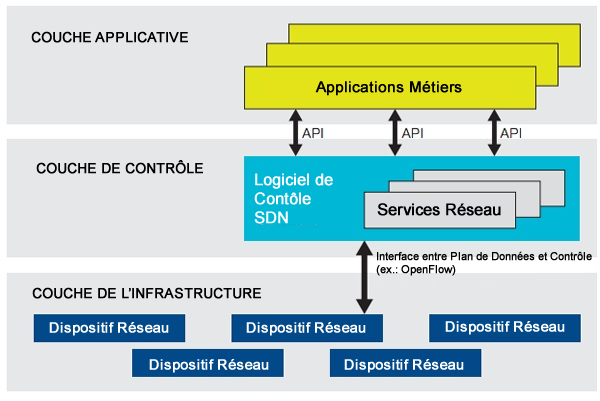
\includegraphics[width=15cm]{images/openflowArchi.jpg} %ou image.png, .jpeg etc.
\caption{ Architecture OpenFlow SDN par ONF \cite{SDNNewNormONFExecutiveSummary}} %la légende
\label{imgArchi} %l'étiquette pour faire référence à cette image
\end{figure} %on ferme l'environnement figure


Les catégories des produits varient aussi en fonction du secteur d'activité des sociétés qui les offrent. En général, les commerçants de chips/silicium proposent des processeurs optimisant la performance du hardware de commutation.  Les vendeurs de switches offrent du matériel capable de communiquer avec un contrôleur SDN. Les spécialistes de la \gls{virtualisation} offrent des solutions logicielles simulant de switchs ou routeurs SDN virtualisés. D'autres sociétés vont investir sur le développement d'un contrôleur SDN. Une pratique adoptée par les géants de l'industrie est l'offre de tout l'écosystème SDN avec souvent un accent sur des applications pour l'automatisation de \gls{datacenter}.\cite{2013GuideSDNNVEcosystem} 
 
 
Le tableau ci-dessous identifie les principaux produits SDN avec leurs respectifs fournisseurs.

\begin{table}[!h]
\centering
\begin{tabular}{|p{6cm}|p{9cm}|}
\hline 
\bf Produit & \bf Vendeur \\ 
\hline 
Puces pour matériel réseau & Boradcom, Intel, Marvell, Mellanox \\ 
\hline 
Switches SDN & Alcatel-Lucent, Avaya, Cisco, Dell, Extreme Networks, HP, NEC, PICA-8, IBM \\ 
\hline 
Systèmes pour la gestion et automatisation du réseau & Packet Design, QualiSystems, EMC, NetScout, CA, HP \\ 
\hline 
Services réseau avec SDN & Embrane, A10, Radware, HP, Riverbed, Citrix, Cisco,  Extreme Networks, NEC \\ 
\hline 
Outils pour la réalisation de tests, les propres résultats des tests & QualiSystems, inCNTRE, Ixia, Spirent \\ 
\hline 
Standards et protocoles & ONF, IEEE, IETF \\ 
\hline 
Contrôleur SDN & Big Switch Networks, NEC, Nuage Networks, Netsocket, HP, Cisco, Open Daylight Consortium, VMware/Nicira \\ 
\hline 
Switchs virtuels et APIs & Citrix, Microsoft, VMWare, Big Switch Networks, Cisco \\ 
\hline 
\end{tabular} 
\caption{Produits SDN et les principaux fournisseurs \cite{2013GuideSDNNVEcosystem}}
\end{table} 
 
Dans les prochaines sections, les offres des principaux acteurs du marché seront présentées.

%%%%%%%Pas exhaustif>>>


\section{Écosystème SDN HP, gamme de solutions virtualisées Data Center}

%Hewlett-Packard executives outlined their software-defined networking (SDN) strategy and position in the market and made a few bets on when the technology will go mainstream. The bet: SDNs will be deployed enterprise-wide in 2015 and represent a \$2 billion market in 2016.
%HP’s argument is that its specialty in automating the data center, as well as a large footprint of customers, make it a leading SDN player.

Les dirigeants de Hewlett-Packard exposent les grandes lignes stratégiques SDN et positionnement face au marché, en pariant sur l'adoption dominante de cette technologie. HP espère que SDN sera largement déployé dans les entreprises en 2015 et qu'il représentera un marché de 2 milliards de dollars en 2016. La société investit dans sa spécialité d'automatisation de \gls{datacenter} pour affirmer sa position de principal acteur SDN. \cite{ExecutiveGuideToSDNHP}


HP a récemment annoncé sa nouvelle gamme de solutions SDN. Avec l'architecture réseau convergé FlexNetwork, HP met en avant son offre jusqu'à deux fois plus évolutive avec 75\% de complexité en moins, par comparaison à d'autres solutions "fabric" proposées sur le marché. En outre, HP affirme que sa solution \gls{fabric} va réduire les délais d’approvisionnement de \gls{datacenter} de quelques mois à seulement quelques minutes. Le portefeuille des services SDN proposés par HP est assez solide, avec des produits ciblant différents points qui vont du traitement des infrastructures existantes à la simplification d'opérations. Par exemple, le HP Virtualized Services Router a été conçu pour éliminer le hardware pouvant être remplacé par des services dans les \glspl{vm}.  

%Hewlett-Packard is stepping up its data center game with a recent announcement of a new suite of solutions for software-defined networking. Built on its FlexNetwork converged networking architecture, HP boasts that it can offer up to two times greater scalability with “75 percent less complexity” compared to other networking fabrics on the market. Furthermore, HP asserted that its data center fabric will reduce provisioning timeframes all the way down from months to mere minutes.


%HP’s portfolio of SDN services is quite substantial, with products aimed at addressing various issues, from dealing with legacy infrastructures to simplifying operations. For example, the HP Virtualized Services Router is designed to cut back data center footprints by delivering services on a virtual machine, which should eliminate “unnecessary hardware.” In addition, the HP HSR 6800 Router Series aims to simplify network service delivery by consolidating routing, firewall, switching, and security onto one device that supports thousands of users. HP’s suite of SDN offerings will be rolling out over the course of the year. Only the HSR 6800 Router Series is available worldwide now, and it holds a starting price of \$46,000. 

La suite d'offres SDN de HP est assez importante, avec des produits qui ciblent divers domaines, l'interopérabilité avec les infrastructures traditionnelles et la simplification des opérations. Par exemple, le produit "HP Virtualized Services Router" est conçu pour éliminer du matériel non essentiel dans les \glspl{datacenter}. De plus, la série "HP HSR 6800 Router Series" a pour but de simplifier la livraison de service réseau en consolidant les fonctions des routage, commutation et sécurité sur le même dispositif supportant des milliers d'utilisateurs. "HP HSR 6800 Router Series" est disponible mondialement au prix initial de \$46,000. \cite{ExecutiveGuideToSDNHPFabric}


%SDN Dev Center.
%SDN App Store.
%HP SDN Developer Kit

\section{Cisco ONE, équipement programmable}

%Cisco also announced it will spend up to \$863 million to acquire Insieme Networks, the company Cisco formed more than a year ago to develop data center networks that are programmable and flexible enough to keep up with the cloud and heavily virtualized data centers.

%The result of Insieme’s work is the Application Centric Infrastructure (ACI), which includes a new line of Nexus 9000 switches that form an application-aware switching fabric along with a centralized controller that manages both virtual and physical network infrastructures.



Cisco a annoncé en novembre 2013 \gls{aci} financée par l'investissement de 863 millions de dollars pour l'acquisition d'Insieme Networks. La start-up développe des réseaux programmables et flexibles pour le cloud et les data centers hautement virtualisés. \gls{aci} est une architecture holistique pour l'automatisation de profils d'application dirigés par politiques centralisés. Le but est d'apporter flexibilité aux logiciels avec \gls{scalability} et performance hardware. 


La solution concrétise \gls{one} qui avait été annoncée précédemment. \gls{one} est une solution complète pour aider les réseaux à devenir plus ouverts, programmables et réactifs aux applications. L'offre inclut une nouvelle ligne de 9000 switches avec un contrôleur capable de gérer les infrastructures physiques et virtuelles. \gls{aci} est disponible sur le marché pour \$75000 avec 288 ports. \cite{CiscoInsiemeLast}


%For now, customers can get into ACI for as low as \$75,000 for 288 ports with a pay-as-you-grow model, said Chambers.


Cisco estime qu'une compréhension approfondie de la couche matérielle est nécessaire. Cela veut dire à la fois que le logiciel et le matériel devraient être développés par la même entreprise et reliés entre eux. À cet effet, Cisco a cherché à embarquer des logiciels très sophistiqués dans ses switches dans le but de renforcer sa crédibilité SDN.
%with centralized automation and policy-driven application profiles. ACI delivers software flexibility with the scalability of hardware performance.
Alors que cette stratégie ne concorde pas tout à fait avec la définition de SDN par \gls{onf}, le résultat obtenu est proche : les switches deviennent plus facilement administrables à travers une interface centrale fournie. Cisco désigne ce modèle comme réseau centré sur les applications, parce que l'organisation introduit des \glspl{api} qui permettent aux applications d'interagir directement avec le réseau. \cite{CiscoSDNONE}

%Cisco refers to this as “application-centric networking” because the company is introducing programmable APIs that allow apps to draw intelligence (and value) directly from the network itself.

%Cisco Open Network Environment (ONE) is a comprehensive solution to help networks become more open, programmable, and application-aware. The broad capabilities of Cisco ONE help meet the needs of numerous market segments, including emerging concepts such as software-defined networking (SDN).

%Cisco believes a thorough understanding of the hardware layer is needed. In turn, this means the software and hardware should be developed by the same company and linked together. To that end, Cisco has so far sought to boost its SDN credibility by embedding more sophisticated software in its switches. While this doesn’t fit the exact definition of SDN—which moves control from switches up into a central management plane, probably using some form of commodity x86 server—it has roughly the same outcome. Switches become more manageable via a central interface.

Cette vision suggère que Cisco tient à s'assurer que cette approche axée logiciel ne menace pas son business consolidé du marché de hardware réseau. Cela permet de maintenir les prix élevés de ces équipements réseau "smarts" tout en permettant de fournir les capacités SDN. Cette approche indique que l'organisation compte embarquer les informations sur les réseaux à partir du matériel vers un logiciel de contrôle plus flexible. Cela diffère de l'approche fédérée par \gls{onf} dont les informations sont diffusées en sens inverse. 

%Cisco’s view, it suggests the company is keen to make sure a more software-focused approach does not threaten its longstanding networking hardware business. For one thing, it lets Cisco keep the prices high on its networking equipment: By using its Cisco ONE (Open Network Environment) technologies to put more software on its switches, it can give customers SDN features while encouraging them to keep on buying its “smart” equipment, which is priced at a premium.

%The approach means Cisco wants to embed information about the network at the hardware layer and have it flow up to a more flexible software control plane. This differs from the approach taken by SDN-like tech- nologies such as OpenFlow and Nicira, which see intelligence originate and reside in the control plane, with decisions pushed out to the hardware.

Finalement, la proposition de Cisco semble valable pour les investisseurs mais potentiellement inintéressante en termes d'innovation technologique. Il est probable que l'entreprise utilise son poids pour chercher à imposer sa vision particulière de SDN en tant qu'un standard. Si cela se produit, les entreprises devront continuer à dépenser de grandes sommes sur du matériel et logiciel propriétaires. Bien que ce scénario puisse rendre SDN plus accessible au début, il risque de devenir contraignant dans le futur. \cite{ExecutiveGuideToSDNCisco}

%Ultimately, Cisco’s approach is good for investors but potentially bad for innovation, as the company will likely seek to use its influence to make its particular view of SDN the industry standard. If this happens, businesses will have to keep spending large amounts of money on IT equipment that dovetails into proprietary software, which then has API compatibility or NIC-support for OpenFlow. Though this may make SDN slightly more ac- cessible to smaller businesses, it could lead to larger companies giving Cisco the cold shoulder and taking the Google route.



\section{Virtualisation : Big Switch Controller et VMWare NSX}

Au sein des vendeurs les plus grands et reconnus, l'innovation peut être plus difficile à atteindre. Ces entreprises ont déjà un modèle de business habituel à maintenir, ce qui est souvent contraignant pour le développement d'une technologie qui est véritablement nouvelle et différente. Pour cette raison SDN a engendré un certain nombre de start-ups avec des technologies porteuses. N'ayant pas cette contrainte, les start-ups spécialisés sur SDN ont eu la liberté de penser au réseau différemment et apporter des produits plus originaux et innovants. Les start-ups dirigent certainement le 'quand' et le 'comment' des innovations sur les réseaux programmables. \cite{startupsSDN}

%SDN has spawned a number of startups with promising technology. The reason for this is that innovation can be harder to come by in the larger, established vendors. The bureaucracy of an established vendor often burdens development teams and can make it nearly impossible to lead with technology that is truly new and different. In addition, large vendors have a customary business model to sustain and shareholders to satisfy each and every quarter. For example, its bottom line is impacted by its ability to push network hardware out the door. Therefore, the SDN strategy focuses on adding new capabilities to that hardware, as that's the least disruptive way to satisfy market demand for SDN without disrupting hardware sales.

%Startup companies have no such inertia. Startups specializing in SDN have exercised their freedom to think about networking in unusual ways and release products that are genuinely new and different. The startups are definitely leading the way when it comes to networking innovation.



Les acquisitions de ces start-ups par les leaders du marché sont devenues assez courantes. VMWare présente sa solution NSX comme une plateforme de virtualisation du réseau pour "software-defined data center". La société a investi 1,3 milliard de dollars dans l'acquisition de Nicira, une entreprise spécialisée dans la virtualisation réseau.
VMWare a intégré sa virtualisation à la technologie Nicira pour faire transiter l'information entre et autour des data centers. L'approche de Nicira est indépendante du hardware et capable de fonctionner comme un contrôleur dans le style SDN. Toutefois, les produits Nicira sont conçus pour gérer les réseaux virtuels plutôt que physiques. \cite{ExecutiveGuideToSDNBigSwitch}


Son principal concurrent est le Big Network Controller, un contrôleur SDN développé par la start-up Big Switch Networks. L'entreprise vise une importante part de marché et s'est fait remarquer par des grands noms. Big Switch a annoncé en novembre son premier produit, un écosystème SDN permettant aux consommateurs de modifier leurs réseaux et data centers via logiciel. La solution est plus large que VMWare NSX et peut menacer aussi le business de fabricants d'équipement réseau, comme Cisco. \cite{BigSwitchLaunchesFirst}
%VMware NSX™ is the network virtualization and security platform for the software-defined data center. NSX brings virtualization to your existing network and transforms network operations and economics. 

%The partners will develop software defined networking (SDN) and network virtualization applications with Big Switch, and will coordinate direct sales efforts with the startup.ranging from traditional network hardware players like Juniper Networks, Arista, Brocade and HP, to hypervisor companies like Citrix and Microsoft

Dans son annonce Big Switch a révélé 27 vendeurs partenaires qui vont développer SDN et des applications virtualisées et coordonner les efforts de ventes directes avec la start-up. Les partenaires varient des traditionnels fabricants de hardware réseau comme Juniper, Brocade et HP à des fabricants d'hyperviseurs comme Citrix et Microsoft. La plateforme proposée offre \gls{fabric} switch OpenFlow qui peut exécuter dans un switch physique ou dans un hyperviseur et permet une large variété d'applications SDN, y compris la virtualisation de data center et réseau ainsi que leur monitoring. \cite{BigSwitchAnnouncement}

%Big Switch Networks is the leader in open source Software-Defined Networking (SDN) products, delivering unmatched network agility, automated network provisioning, and dramatic reductions in the cost of network operations. The company’s Open SDN™ platform offers an OpenFlow switch fabric that can run on bare metal switches and hypervisor virtual switches, and enables a wide variety of SDN network applications including data center network virtualization and network monitoring. 

%VMware made a splash with its acquisition of Nicira, and SDN acquisitions have become common.
%VMware has acquired network virtualisation company Nicira for \$1.3bn.

%VMware is expected to integrate Nicira’s technology with its virtualisation software to help move information around and between data centers. Crucially, Nicira’s approach does not care about the underlying hardware. This means that Nicira-based networks are not tied to any one supplier and are capable of an SDN-style central control plane.

%Nicira’s products are designed to manage virtual networks rather than physical ones.




%\section{Brocade Ethernet Fabric, Fibre Channel support over Ethernet}
%Virtual Cluster Switching
%Pour les architectes du réseau et serveurs de data centre.


%\section{Juniper MetaFabric Architecture}

%\section{Citrix NetScaler, plate-forme ouverte dirigée par app }


\addchap{Conclusion}

Même avec le succès incontestable de l'architecture d'internet, l'état de l'industrie réseau et l'essence de son infrastructure se retrouvent en phase critique. Il est généralement admis que les réseaux courants sont excessivement chers, compliqués à gérer, sujets aux blocages des fournisseurs et difficiles à faire évoluer. 

En effet, on constate un réel besoin de faire évoluer cette architecture mais aussi des résistances contraignant cette évolution dues à la complexité et la possible saturation du système. En réponse, les réseaux programmables ont été objet intensif de recherche par la communauté. Les travaux dans le domaine ont progressé vers la proposition de SDN, un nouveau paradigme transformant cette architecture.

L'approche SDN découpe le plan de contrôle et le plan données, offrant un contrôle et une vision centralisés du réseau. Cela peut apporter certains bénéfices comme le contrôle directement programmable, la simplification du hardware réseau et la simplification de l'ingénierie du trafic. En revanche, des challenges d'implémentation sont à surmonter tels que la concentration des risques dans un contrôle physiquement centralisé, l'équilibre entre flexibilité et performance et les conditions d'interopérabilité.

La flexibilité apportée par SDN est telle que de nombreuses possibilités d'applications sont à imaginer. Essentiellement le management de data centers, le contrôle d'accès et de la mobilité pour les réseaux campus ainsi que  l'ingénierie du trafic pour les réseaux WAN.

Le marché suit de près les nouveautés dans le domaine et investit sur les technologies implémentant SDN. Les stratégies sont pas encore assez matures et les potentiels consommateurs attendent des offres plus consolidées. Cependant, des solutions innovantes commencent à surgir et certaines organisations assument un rôle de tête dans le marché.

On s'aperçoit que l'ampleur des possibilités SDN même si un avantage en théorie, frein son adoption. Dû à la massive variété des concepts et produits, les consommateur hésitent toujours à prendre des décisions. Au même temps, les grands fournisseurs cherchent à la fois à exploiter le nouveau marché et à protéger leurs solutions consolidées. Cet impasse même si confirmé, ne semble pas être assez fort pour empêcher les échanges à long terme.

En caractère personnel, cette étude conclue qu'au futur proche, les clients les plus informés et les plus prêt à innover vont commencer à déployer SDN. Vu que leurs expériences et résultats peuvent fortement impacter les choix des prochains consommateurs, il est possible que les premiers à se lancer seront ceux qui vont peindre le futur de la technologie des réseaux informatiques pour les prochaines années. Cette démarche peut représenter un risque au cas échéant, mais aussi l'opportunité d'en tirer des bénéfices plus durables et de prendre de parts plus larges du marché.

\appendix
\chapter{Première annexe}


%\include{ann2}
%\gls{sdn}
%\gls{paradigme}
\gls{ti}

\backmatter
\nocite{*}
\printbibliography
\printindex

\glsaddall
\printglossaries

\cleardoublepage
\includepdf[pages={3-4}]{couverture-ebt.pdf}
\end{document}
